\documentclass[12pt,letterpaper]{article}
\usepackage[body={18cm, 25cm}]{geometry}
\usepackage[spanish, activeacute]{babel}
\usepackage[utf8]{inputenc}
\decimalpoint
\usepackage{natbib}
\usepackage{lscape}
\usepackage{amsmath}
\usepackage{amsfonts}
\usepackage{amssymb}
\usepackage{graphicx}
\usepackage{geometry}
\usepackage{float}
%\usepackage{subfloat}
\usepackage{caption}
\usepackage{subcaption}
\usepackage{algpseudocode}
%\usepackage{subfig}%%Para incluir subgraficos
\usepackage{fancyhdr}%%Para incluir encabezado
\usepackage[pdftex, pdftitle={Rotación de Vectores}, pdfauthor={J. Vergara}, pdfsubject={Vectors}, pdfkeywords={vectores, rotación, mecánica del medio continuo}, pdfpagemode=UseOutlines,bookmarks,bookmarksopen,pdfstartview=FitH,colorlinks,linkcolor=blue, urlcolor=black, citecolor=blue]{hyperref}
\geometry{verbose,letterpaper,tmargin=3cm,bmargin=3cm,lmargin=3cm,rmargin=3cm}


\author{Juan Carlos Vergara Gallego - Grupo de Investigación en Mecánica Aplicada \\ Universidad EAFIT}
\title{\textbf{Rotación de Vectores, Caso $2D$ y $3D$}}

\usepackage{cleveref}
\begin{document}

\pagestyle{fancyplain}
\fancyhf{}
%\fancyheadoffset[LE,RO]{\marginparsep+\marginparwidth}
\headheight=20pt %para cambiar el tamaño del encabezado
\renewcommand{\headrulewidth}{0pt} %espesor del encabezado

\lhead %la "L" indica a la izquierda
{
\begin{minipage}{3cm}

\includegraphics[width=1.5 in]{img/logo.pdf}
\end{minipage}
}

\fancyfoot[c]{\thepage}

\maketitle


{\bf Palabras clave:} Vectores, Rotación, Mecánica del Medio Continuo.\\\\

\abstract
%
En este documento se presenta la formulación mediante la cual se hace posible describir un vector que se encuentra descrito en un sistema de referencia $x-y-z$ en otro sistema de referencia $x'-y'-z'$.
%
\section{Planteamiento del problema}
%
En la figura \ref{planteamiento} se presenta la descripción gráfica del problema, el cual corresponde en encontrar la relación matemática para expresar un vector que se encuentra descrito en el sistema de referencia $x-y$ al sistema de referencia $x'-y'$. En esta figura se presentan los ángulos entre cada uno de los ejes de los sistemas de referencia y los vectores unitarios base de cada sistema de referencia.\\
%
\begin{figure}[h]
	\centering
	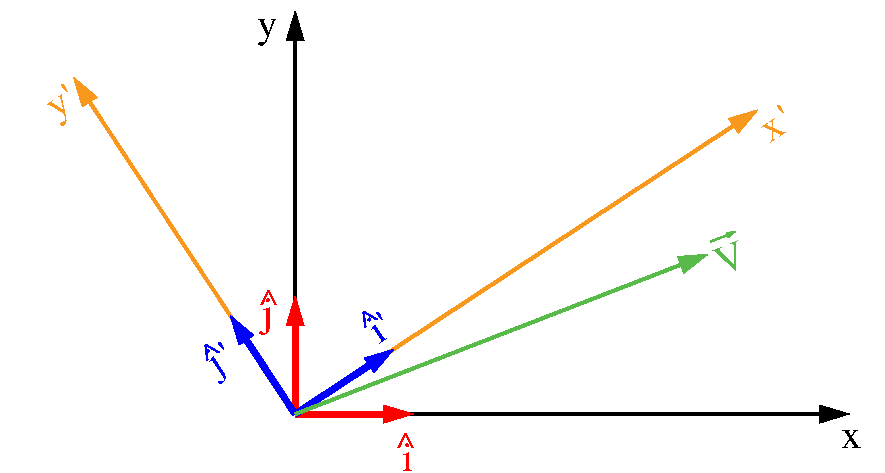
\includegraphics[width=8cm]{img/Planteamiento.pdf}
	\caption{Ángulos entre los ejes de ambos sistemas de referencia.}
	\label{planteamiento}
\end{figure}
%
\begin{itemize}
	\item $\theta_{x-x'}$: Ángulo entre el eje $x$ y $x'$
	\item $\theta_{x-y'}$: Ángulo entre el eje $x$ y $y'$
	\item $\theta_{y-x'}$: Ángulo entre el eje $y$ y $x'$
	\item $\theta_{y-y'}$: Ángulo entre el eje $y$ y $y'$
	\item $\hat{i}$, $\hat{j}$: Vectores unitarios bases del sistema de referencia $x-y$.
	\item $\hat{i}'$, $\hat{j}'$: Vectores unitarios bases del sistema de referencia $x'-y'$.
\end{itemize}
%
%
\section{Desarrollo del problema $2D$}
%
En la figura \ref{vector1} y \ref{vector2} se presenta el vector $\overset{\rightarrow}{V}$ en los sistemas de referencia $x-y$ y $x'-y'$ respectivamente.\\
%
%
\begin{figure}[h]
	\centering
	\begin{subfigure}[l]{0.450\textwidth}
		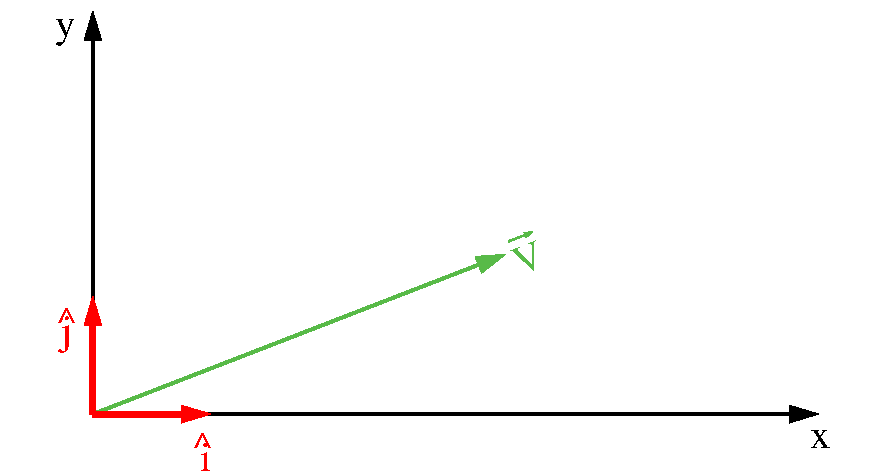
\includegraphics[width=\textwidth]{img/Vector1.pdf}
		\caption{Vector $\overset{\rightarrow}{V}$ en el sistema de referencia $x-y$.}
		\label{vector1}
	\end{subfigure}
	\hspace{.5 cm}
	%
	\begin{subfigure}[r]{0.450\textwidth}
		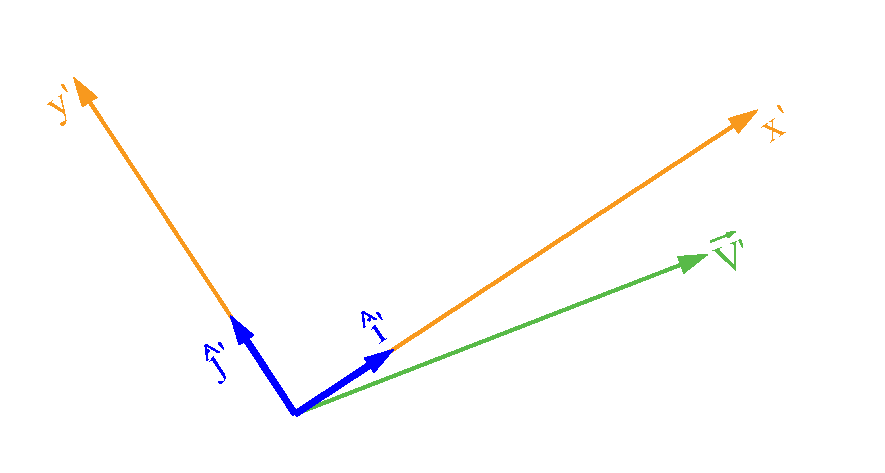
\includegraphics[width=\textwidth]{img/Vector2.pdf}
		\caption{Vector $\overset{\rightarrow}{V'}$ en el sistema de referencia $x'-y'$.}
		\label{vector2}
	\end{subfigure}	
	\caption{}
\end{figure}
%
%
El vector $\overset{\rightarrow}{V}$ y $\overset{\rightarrow}{V'}$ son el mismo en ambos sistemas de referencia, su magnitud y significado físico no varía por tener diferente sistema de referencia, lo único diferente entre estos es la forma de representarlos en terminos de sus componentes. Lo cual se puede escribir matemáticamente como:
%
\begin{align}
	\overset{\rightarrow}{V} = \overset{\rightarrow}{V'}
	\label{uno}
\end{align}
%
Dónde:
%
\begin{align}
	\overset{\rightarrow}{V} = V_x \hat{i} + V_y \hat{j} \label{dos}\\
	\overset{\rightarrow}{V'} = V_{x'} \hat{i'} + V_{y'} \hat{j'} \label{tres}
\end{align}
%
Ahora, expresamos el vector unitario $\hat{i}$ en términos de los vectores unitarios $\hat{i}'$ y $\hat{j}'$, luego hacemos lo mismo con el vector unitario $\hat{j}$.
%
\begin{align}
	\hat{i} = \hat{i}' \cos \theta_{x-x'} +  \hat{j}' \cos \theta_{x-y'} \label{cuatro}\\
	\hat{j} = \hat{i}' \cos \theta_{y-x'} +  \hat{j}' \cos \theta_{y-y'} \label{cinco}
\end{align}
%
Reemplazando las ecuaciones \ref{cuatro} y \ref{cinco} en la ecuación \ref{dos}:
%
\begin{align*}
	\overset{\rightarrow}{V} = V_x \left( \hat{i}' \cos \theta_{x-x'} + \hat{j}' \cos \theta_{x-y'} \right) + V_y \left( \hat{i}' \cos \theta_{y-x'} + \hat{j}' \cos \theta_{y-y'} \right)
\end{align*}
%
Reorganizando los términos:
%
\begin{align}
	\overset{\rightarrow}{V} = \left( V_x \cos \theta_{x-x'} + V_y \cos \theta_{y-x'} \right) \hat{i}'+ \left( V_x \cos \theta_{x-y'} + V_y \cos \theta_{y-y'} \right) \hat{j}' \label{seis}
\end{align}
%
Ahora reemplazamos las ecuaciones \ref{seis} y \ref{tres} en la ecuación \ref{uno}:
%
\begin{align}
	\left( V_x \cos \theta_{x-x'} + V_y \cos \theta_{y-x'} \right) \hat{i}'+ \left( V_x \cos \theta_{x-y'} + V_y \cos \theta_{y-y'} \right) \hat{j}' = V_{x'} \hat{i}' + V_{y'} \hat{j}' \label{siete}
\end{align}
%
Ambos lados de la ecuación \ref{siete} contiene términos que dependen de $\hat{i}'$
y $\hat{j}'$. Igualando los términos que dependen de $\hat{i}'$ y los que dependen de $\hat{j}'$, llegamos a:
%
\begin{align}
	V_x \cos \theta_{x-x'} + V_y \cos \theta_{y-x'} = V_{x'} \label{ocho}\\
	V_x \cos \theta_{x-y'} + V_y \cos \theta_{y-y'} = V_{y'} \label{nueve}
\end{align}
%
Las ecuaciones \ref{ocho} y \ref{nueve} las expresamos matricialmente:
%
\begin{eqnarray}
		\left[ \begin{array}{c} V_{x'} \\
		V_{y'} \end{array} \right] = 
		\left[ \begin{array}{cc}
		\cos \theta_{x-x'} & \cos \theta_{y-x'} \\  
		\cos \theta_{x-y'} & \cos \theta_{y-y'}
		\end{array}  \right] 
		\left[ \begin{array}{c} V_{x} \\
		V_{y} \end{array} \right]
		\label{diez}
\end{eqnarray}
%
En la ecuación \ref{diez} se identifican los siguientes elementos:
%
\begin{align*}
	\left[ \begin{array}{c}
		V_x \\
		V_y	
	\end{array} \right]: \textup{Componentes del vector $\overset{\rightarrow}{V}$ en el sistema de referencia $x-y$} 
\end{align*}
%
\begin{align*}
	\left[ \begin{array}{c}
		V_{x'} \\
		V_{y'}	
	\end{array} \right]: \textup{Componentes del vector $\overset{\rightarrow}{V'}$ en el sistema de referencia $x'-y'$} 
\end{align*}
%
\begin{align}
	\left[ T \right] = \left[ \begin{array}{cc}
		\cos \theta_{x-x'} & \cos \theta_{y-x'} \\
		\cos \theta_{x-y'} & \cos \theta_{y-y'}	
	\end{array} \right] \label{once}
\end{align}
%
La  ecuación \ref{once} corresponde a la matriz de transformación, la cual nos permite representar entidades físico-matemáticas, descritas en el sistema de referencia $x-y$, en el sistema de referencia $x'-y'$.\\\\
%
¿Cómo leer y/o hallar la matriz de transformación $\left[ T \right]$?.\\\\
%
Lectura de columnas:
%
\begin{itemize}
	\item Columna 1: $ \left[ \begin{array}{c}
		\cos \theta_{x-x'} \\	 \cos \theta_{x-y'}
	\end{array} \right]$, vector que contiene los cosenos de los ángulos entre el eje $x$ del sistema de referencia original y los ejes $x'$ y $y'$ (ver figura \ref{planteamiento}).
	\item Columna 2: $ \left[ \begin{array}{c}
		\cos \theta_{y-x'} \\	 \cos \theta_{y-y'}
	\end{array} \right]$, vector que contiene los cosenos de los ángulos entre el eje $y$ del sistema de referencia original y los ejes $x'$ y $y'$ (ver figura \ref{planteamiento}).
\end{itemize}
%
Lectura de filas:
%
\begin{itemize}
	\item Fila 1: $ \left[ \begin{array}{cc}
		\cos \theta_{x-x'} &	 \cos \theta_{y-x'}
	\end{array} \right]$, vector que contiene los cosenos de los ángulos entre los ejes $x$ y $x'$ y entre los ejes $y$ y $x'$ (ver figura \ref{planteamiento}).
	\item Fila 2: $ \left[ \begin{array}{cc}
		\cos \theta_{x-y'} &	 \cos \theta_{y-y'}
	\end{array} \right]$, vector que contiene los cosenos de los ángulos entre los ejes $x$ y $y'$ y entre los ejes $y$ y $y'$ (ver figura \ref{planteamiento}).
\end{itemize}
%
Si lo que conocemos es el vector en el sistema de referencia $x'-y'$ y lo queremos expresar en el sistema de referencia $x-y$, solo es necesario realizar manipulaciones matemáticas simples sobre la ecuación \ref{diez}.\\
%
Reescribiendo la ecuación \ref{diez}:
%
\begin{align*}
	\left[ V' \right] = \left[ T \right] \left[ V \right]
\end{align*}
%
Premultiplicamos la ecuación \ref{diez} por la inversa de la matriz de transformación:
%
\begin{align*}
	\left[ T \right]^{-1} \left[ V' \right] = \left[ T \right]^{-1} \left[ T \right] \left[ V \right]
\end{align*}
%
Ya que $\left[ T \right]$ es una matriz de transformación entre dos sistemas de referencia ortogonales, se tiene que $\left[ T \right]^{-1} = \left[ T \right]^T$. Además, se tiene que $\left[ T \right] \left[ T \right]^T = \left[ I \right]$ y que $\left[ I \right] \left[ V \right] = \left[ V \right]$.
%
\begin{align}
	\left[ V \right] = \left[ T \right]^T \left[ V' \right] \label{doce}
\end{align}
%
La ecuación \ref{doce} nos permite expresar el vector $\overset{\rightarrow}{V'}$ del sistema de referencia $x'-y'$ en el sistema de referencia $x-y$.\\\\
%
{\bf Nota importante: } Se utiliza la función trigonométrica {\it{Coseno}} pues esta es una función par y por ende no importa el signo del ángulo entre los ejes.\\
$\cos \left( -\theta \right) = \cos \left( \theta \right)$
%
%
\section{Desarrollo del problema $3D$}
%
El caso tridimensional $(3D)$ no es nada más que una extensión del caso bidimensional $(2D)$, por lo cual en este documento solo se muestra que se le debe adicionar a las ecuaciones descritas en el caso $(2D)$.
%
\begin{itemize}
	\item $\theta_{x-x'}$: Ángulo entre el eje $x$ y $x'$
	\item $\theta_{x-y'}$: Ángulo entre el eje $x$ y $y'$
	\item $\theta_{x-z'}$: Ángulo entre el eje $x$ y $z'$
	\item $\theta_{y-x'}$: Ángulo entre el eje $y$ y $x'$
	\item $\theta_{y-y'}$: Ángulo entre el eje $y$ y $y'$
	\item $\theta_{y-z'}$: Ángulo entre el eje $y$ y $z'$
	\item $\theta_{z-x'}$: Ángulo entre el eje $z$ y $x'$
	\item $\theta_{z-y'}$: Ángulo entre el eje $z$ y $y'$
	\item $\theta_{z-z'}$: Ángulo entre el eje $z$ y $z'$
	\item $\hat{i}$, $\hat{j}$, $\hat{k}$: Vectores unitarios bases del sistema de referencia $x-y-z$.
	\item $\hat{i}'$, $\hat{j}'$, $\hat{k}'$: Vectores unitarios bases del sistema de referencia $x'-y'-z'$.
\end{itemize}
%
Reescribimos la ecuación \ref{diez}:
%
\begin{eqnarray}
		\left[ \begin{array}{c} V_{x'} \\
		V_{y'} \\ V_{z'} \end{array} \right] = 
		\left[ \begin{array}{ccc}
		\cos \theta_{x-x'} & \cos \theta_{y-x'} & \cos \theta_{z-x'} \\  
		\cos \theta_{x-y'} & \cos \theta_{y-y'} & \cos \theta_{z-y'} \\
		\cos \theta_{x-z'} & \cos \theta_{y-z'} & \cos \theta_{z-z'}
		\end{array}  \right] 
		\left[ \begin{array}{c} V_{x} \\
		V_{y} \\ V_{z} \end{array} \right]
		\label{trece}
\end{eqnarray}
%
Donde:
%
\begin{align}
	\left[ T \right] = \left[ \begin{array}{ccc}
		\cos \theta_{x-x'} & \cos \theta_{y-x'} & \cos \theta_{z-x'} \\  
		\cos \theta_{x-y'} & \cos \theta_{y-y'} & \cos \theta_{z-y'} \\
		\cos \theta_{x-z'} & \cos \theta_{y-z'} & \cos \theta_{z-z'}
		\end{array}  \right] \label{catorce}
\end{align}
%
El significado de las columnas y filas de la matriz de transformación $\left[ T \right]$ de la ecuación \ref{catorce} es el mismo al que se le dio para el caso de la matriz de transformación presentada en la ecuación \ref{once}.\\\\
%
Reescribiendo la ecuación \ref{trece} en forma compacta y la ecuación de transformación de $x'-y'-z'$ a $x-y-z$.
%
\begin{align*}
	\left[ V' \right] = \left[ T \right] \left[ V \right] \\
	\left[ V \right] = \left[ T \right]^T \left[ V' \right]
\end{align*}
%
%
\end{document}